% Chapter Template

\chapter{Introduction and Background} % Main chapter title

\label{Chapter1} % Change X to a consecutive number; for referencing this chapter elsewhere, use \ref{ChapterX}

\lhead{Chapter 1. \emph{Introduction and Background}} % Change X to a consecutive number; this is for the header on each page - perhaps a shortened title

%----------------------------------------------------------------------------------------
%	SECTION 1
%----------------------------------------------------------------------------------------

\section{Wind Power}

Wind power is the fastest growing energy source in the world.  From 2000 to 2015, global wind power capacity grew from 17,400MW to 432,883MW, with an average increase of 24\% per year (Figure \ref{fig1-1} ). In 2015, the increase in wind generation was equal to almost half of global electricity growth\cite{sawyer2015}. In the United States, installed wind capacity grew from approximately 2,500 MW in the year 2000 to 82,143 MW in 2016 \cite{williams2016}. Though wind power only represents a small fraction of total global power generation, it is an important source of clean renewable energy and its importance will increase in the future.

\begin{figure}[htbp]
	\centering
		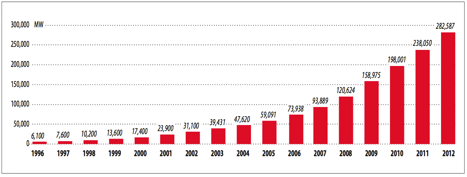
\includegraphics[width=\linewidth]{Figures/ch1Figures/fig1-1.png}
	\caption{Global wind power capacity. \cite{sawyer2015}}
	\label{fig1-1}
\end{figure}

Much of wind power$'$s success is due to two factors: the widespread availability of wind resources and the relatively low Cost of Energy (COE) when compared to other renewable energy sources.  For example, utility scale wind energy typically costs 5-12 cents per KW-hr while utility scale solar-PV typically costs 15-30 cents per KW-hr \cite{ren212011}. Though some renewable energy sources such as geothermal plants or large hydro plants can produce energy at lower COE than wind farms, the natural resources needed for those plants are much more limited.  

The cost of wind power has been steadily decreasing.  The decreases in wind power COE have gone hand in hand with increases in both the size and complexity of wind turbines.  As the turbines have grown in size and complexity, more sophisticated methods for controlling those turbines have been required.  


%----------------------------------------------------------------------------------------
%	SECTION 2
%----------------------------------------------------------------------------------------

\section{Wind Turbine Control} \label{section1-2} 

A control system typically consists of sensors, actuators, and a controller. A modern wind turbine might include sensors such as: an anemometer, a wind vane, at least one rotor speed sensor, an electric power sensor, accelerometers, load sensors, pitch position sensors, various limit switches, vibration sensors, temperature and oil level indicators, hydraulic pressure sensors, operator switches, and push buttons.  Actuators might include:  hydraulic or electric pitch actuators, an electric generator that can actively control generator torque, generator contacts, switches for activating shaft brakes, and yaw motors.  The controller collects information from sensors, processes that data, the issues commands to actuators. For a wind turbine, the controller typically consists of a computer based controller used for normal operation, and a highly reliable hard wired safety system that overrides the computer based controller and brings the turbine to a safe state if a serious problem occurs.\cite{burton2011}

The control system performs a variety of functions, but this research is primarily concerned with the closed loop control system that optimizes turbine performance during power production. The majority of utility scale turbines built today use variable speed and collective pitch to feather control.  In this control scheme both the rotational speed of the turbine and the collective pitch of the turbine$'$s three blades are controlled. At low and medium wind speeds the pitch is held constant while the turbine speed is varied.  At high wind speeds both the turbine speed and the blade pitch can be varied.

At low and medium wind speeds, the rotational speed of the rotor is manipulated to maximize aerodynamic efficiency and maximize energy capture.  The variations in rotational speed are achieved by torque control, which is implemented by using a pre-determined generator torque vs. generator speed curve like the one shown in Figure \ref{fig1-2}.  The torque controller receives measurements from a generator speed sensor, looks up the appropriate generator torque on the speed-torque curve and commands the generator to produce that torque. The blue line in Figure \ref{fig1-2} shows the torque vs. speed curve for the torque controller on the NREL 5-MW reference turbine.  The black line shows the torque-speed curve corresponding to maximum aerodynamic efficiency of the turbine. Figure \ref{fig1-3} shows the relationship between generator speed and generated power. In region 1 the generator produces no torque and no power, in region 2 the generator tracks optimum aerodynamic efficiency, and in region 3 the generator tracks constant power output.  Regions 1.5 and 2.5 simply serve as smooth transitions between the other regions. 



\begin{figure}[htbp]
	\centering
		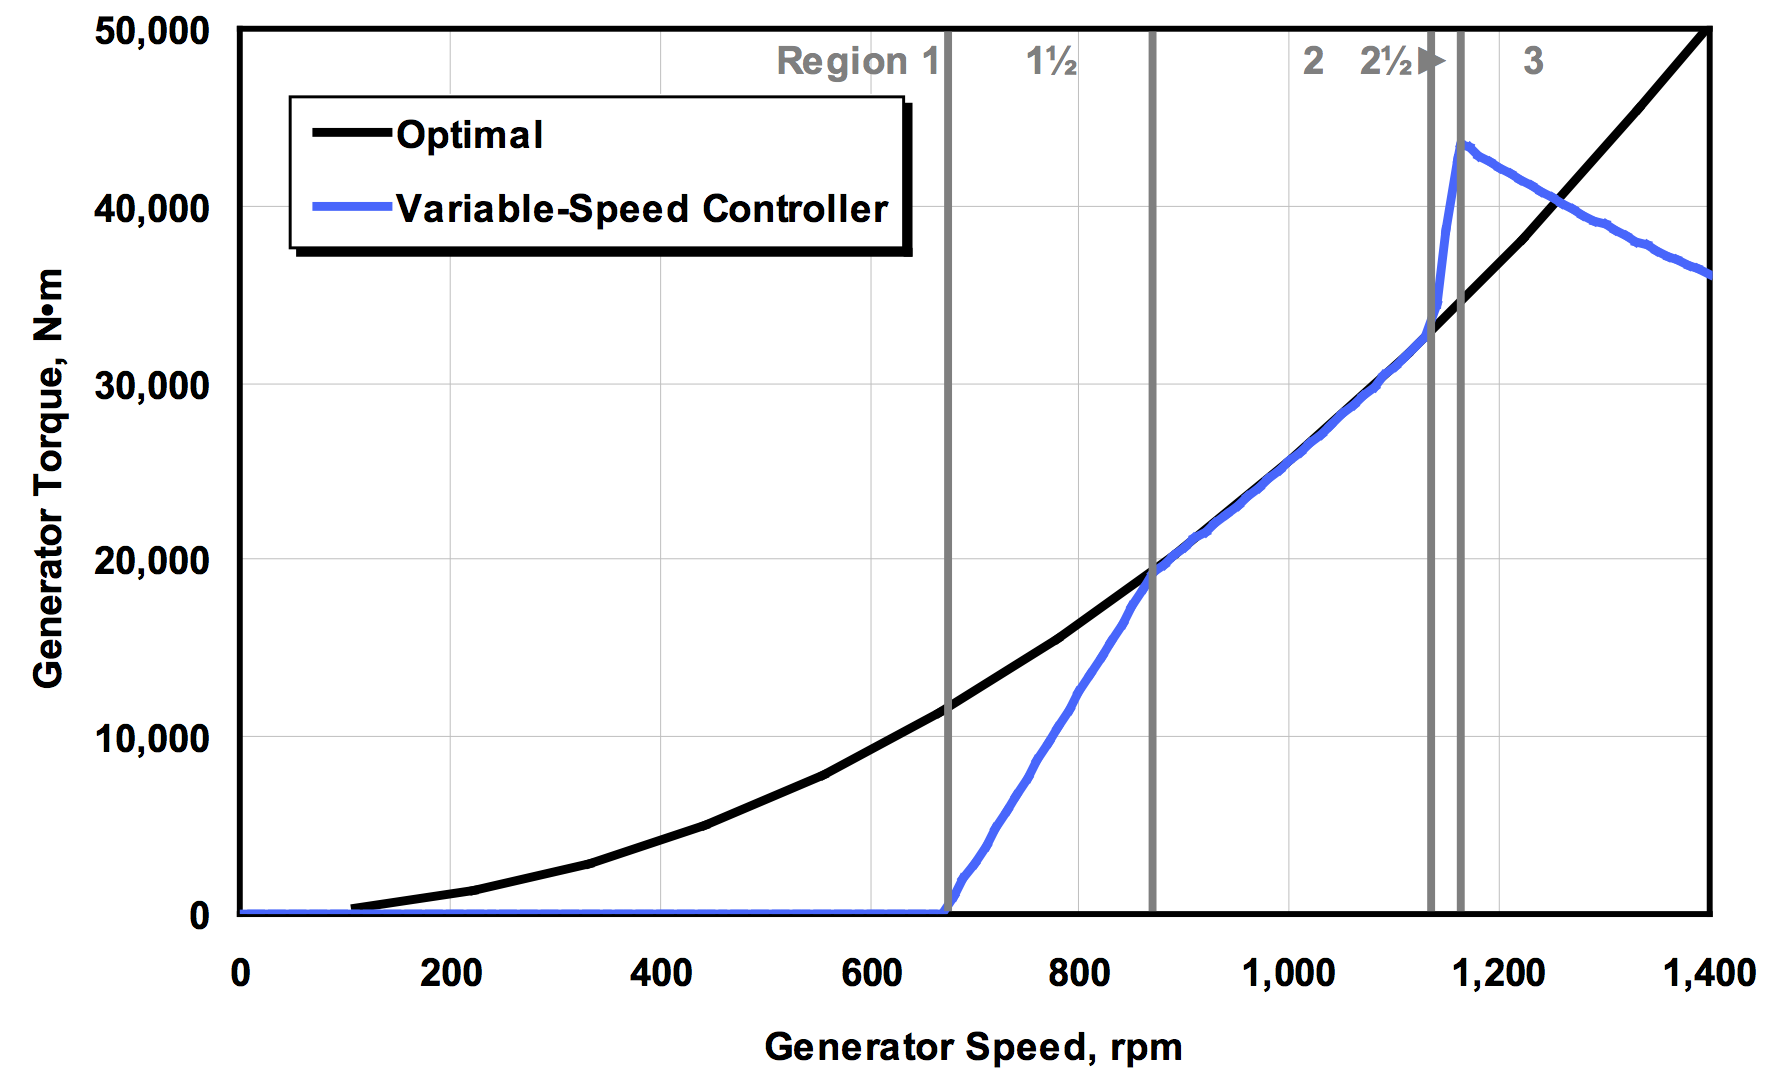
\includegraphics[width=.75\linewidth]{Figures/ch1Figures/fig1-2.png}
	\caption{Torque-speed curve for NREL 5-MW turbine.\cite{jonkman2009}}
	\label{fig1-2}
\end{figure}

\begin{figure}[htbp]
	\centering
		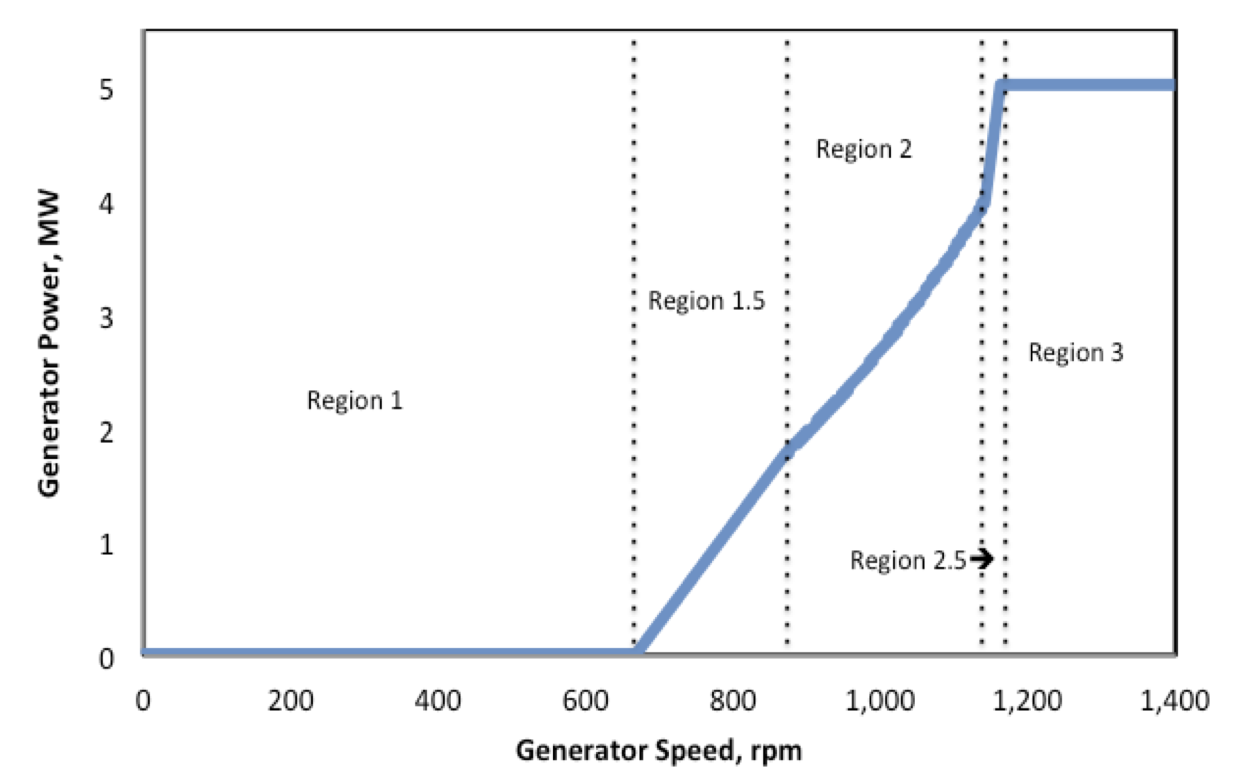
\includegraphics[width=.75\linewidth]{Figures/ch1Figures/fig1-3.png}
	\caption{Power-speed curve for NREL 5-MW turbine.}
	\label{fig1-3}
\end{figure}

At high wind speeds the collective blade pitch is manipulated to keep turbine speed and power generation constant. As wind speed increases, the turbine blades are pitched such that the turbine extracts a smaller fraction of the wind$'$s power.  As a result, the turbine is able to maintain the same power production even as the total available power in the wind increases.  The purpose of pitch control is to manage loading on the turbine$'$s mechanical components, and to prevent the turbine$'$s power electronics from being damaged by excessive power production.   For the NREL 5-MW turbine pitch control is achieved with a nonlinear PI controller in which the controller gains vary depending on the current blade pitch angle. 

%----------------------------------------------------------------------------------------
%	SECTION 3
%----------------------------------------------------------------------------------------

\section{Advanced Turbine Control Research} 

The advanced wind turbine control concepts being researched today are numerous and diverse. A comprehensive review of this field is outside the scope of this proposal, but in the following paragraphs I will briefly describe several areas of advanced wind turbine control that are related to the work in this thesis: Individual pitch control, active load control, and LIDAR assisted control.

In individual pitch control, the pitch of each turbine blade is controlled independently and the blades can be set at different pitch angles.  This has several advantages over the collective pitch control described in the previous section. Individual pitch control can be used to reduce loading caused by rotor tilt and yaw alignment errors, airflow effects caused by wind turbine tower, or any other loads that vary cyclically with the rotation of the blade. Research has shown that cyclic pitch control could lead to a 30-40\% reduction in fatigue loads on the turbine hub and a 20-30\% reduction in fatigue loads at the blade roots.\cite{larsen2005,bossanyi2004} However, there is concern that the additional pitching will lead to premature failure of the blade pitching mechanism, or that it will require larger, more costly blade pitching mechanisms.\cite{vandam2008}

Active flow control is the control of local airflow surrounding the blade.  In the past, a great deal of research has focused on active flow control for aircraft. Recent research has sought to apply active flow technologies to commercial wind turbines as well. Active flow control typically operates on a small scale.  It uses devices, such as the red trailing edge flaps shown in Figure \ref{fig1-4}, to exercise local control over the aerodynamic properties of the blade.  These devices can independently control the aerodynamic properties of small portions of a wind turbine blade.  The devices also typically have very quick response times.  Because they respond quickly and because they can exercise local control over smaller portions of the turbine blade, active flow control devices have the potential to mitigate some loads that other control methods cannot.  



\begin{figure}[ht]
	\centering
		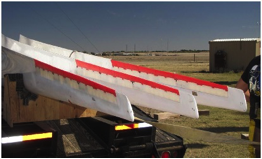
\includegraphics[width=.75\linewidth]{Figures/ch1Figures/fig1-4.png}
	\caption{Wind turbine blades with trailing edge flaps for active load control.\cite{berg2012}}
	\label{fig1-4}
\end{figure}

In LIDAR assisted control a LIDAR (Light Detection and Ranging) system is mounted on the nacelle of a turbine and used to scan the wind field as it approaches the wind turbine.  As illustrated in Figure \ref{fig1-5}, the LIDAR system is capable of measuring wind speed at several discrete distances upwind of the turbine.  These measurements are used to estimate the wind speed that the turbine will experience in the future.  The turbine controller can use these future wind speed estimates to respond preemptively to changes in wind speed and to counteract changes in aerodynamic loading as they occur. The primary disadvantage to LIDAR control is the prohibitive cost of the LIDAR equipment.  

\begin{figure}[ht]
	\centering
		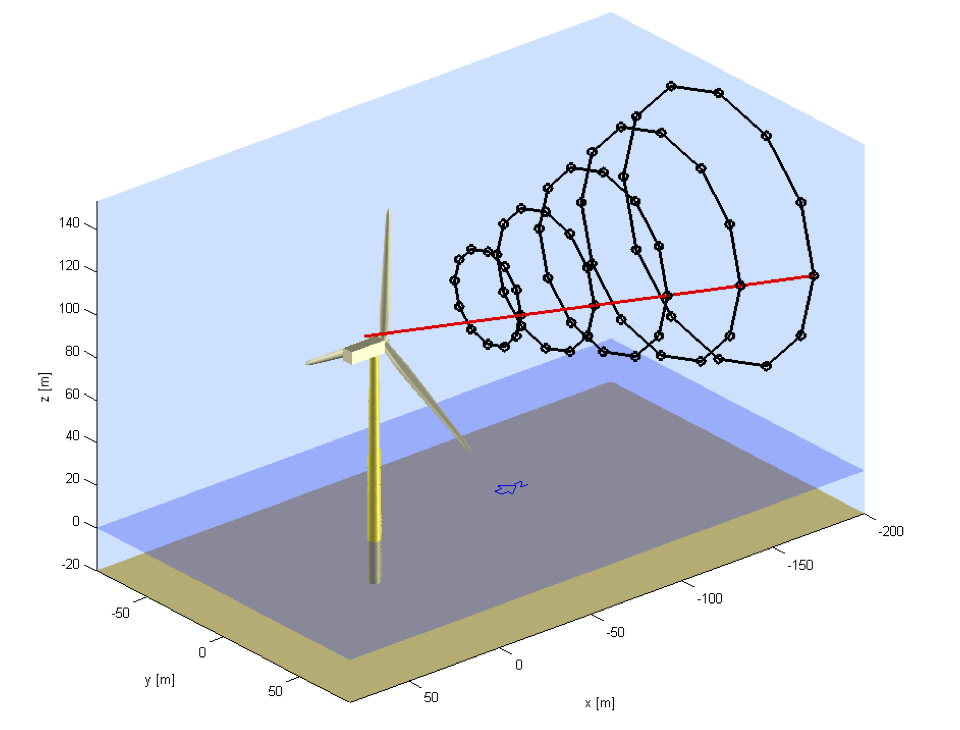
\includegraphics[width=.6\linewidth]{Figures/ch1Figures/fig1-5.png}
	\caption{Illustration of upwind LIDAR measurement distances.\cite{schlipf2011}}
	\label{fig1-5}
\end{figure}

%----------------------------------------------------------------------------------------
%	SECTION 4
%----------------------------------------------------------------------------------------

\section{Goals of This Research} 

This dissertation seeks to improve wind turbine control by using information obtained from upwind turbines.  In particular, pre-existing sensors on upwind turbines will measure wind speed fluctuations and dynamic turbine behavior.  That information will then be used by the control system of a downwind turbine to anticipate wind speed fluctuations before they reach the downwind turbine.  This technique holds the potential to improve power production and/or decrease turbine loads by allowing the downwind turbine to react preemptively to changes in wind speed and track the optimum turbine conditions more closely.

Figure \ref{fig1-6} shows the steady state power curve for the NREL 5-MW turbine.  It represents the optimum power production at each wind speed.  If the wind blows at a constant speed for long enough, the control system will bring the turbine$'$s power production to a point on the blue line.  However, since rapid wind speed fluctuations are common, the turbine often deviates from this power curve during normal operation.  If the magnitude and/or time of these deviations can be reduced then the power curve can be tracked more closely and several potential benefits can be achieved.


\begin{figure}[htbp]
	\centering
		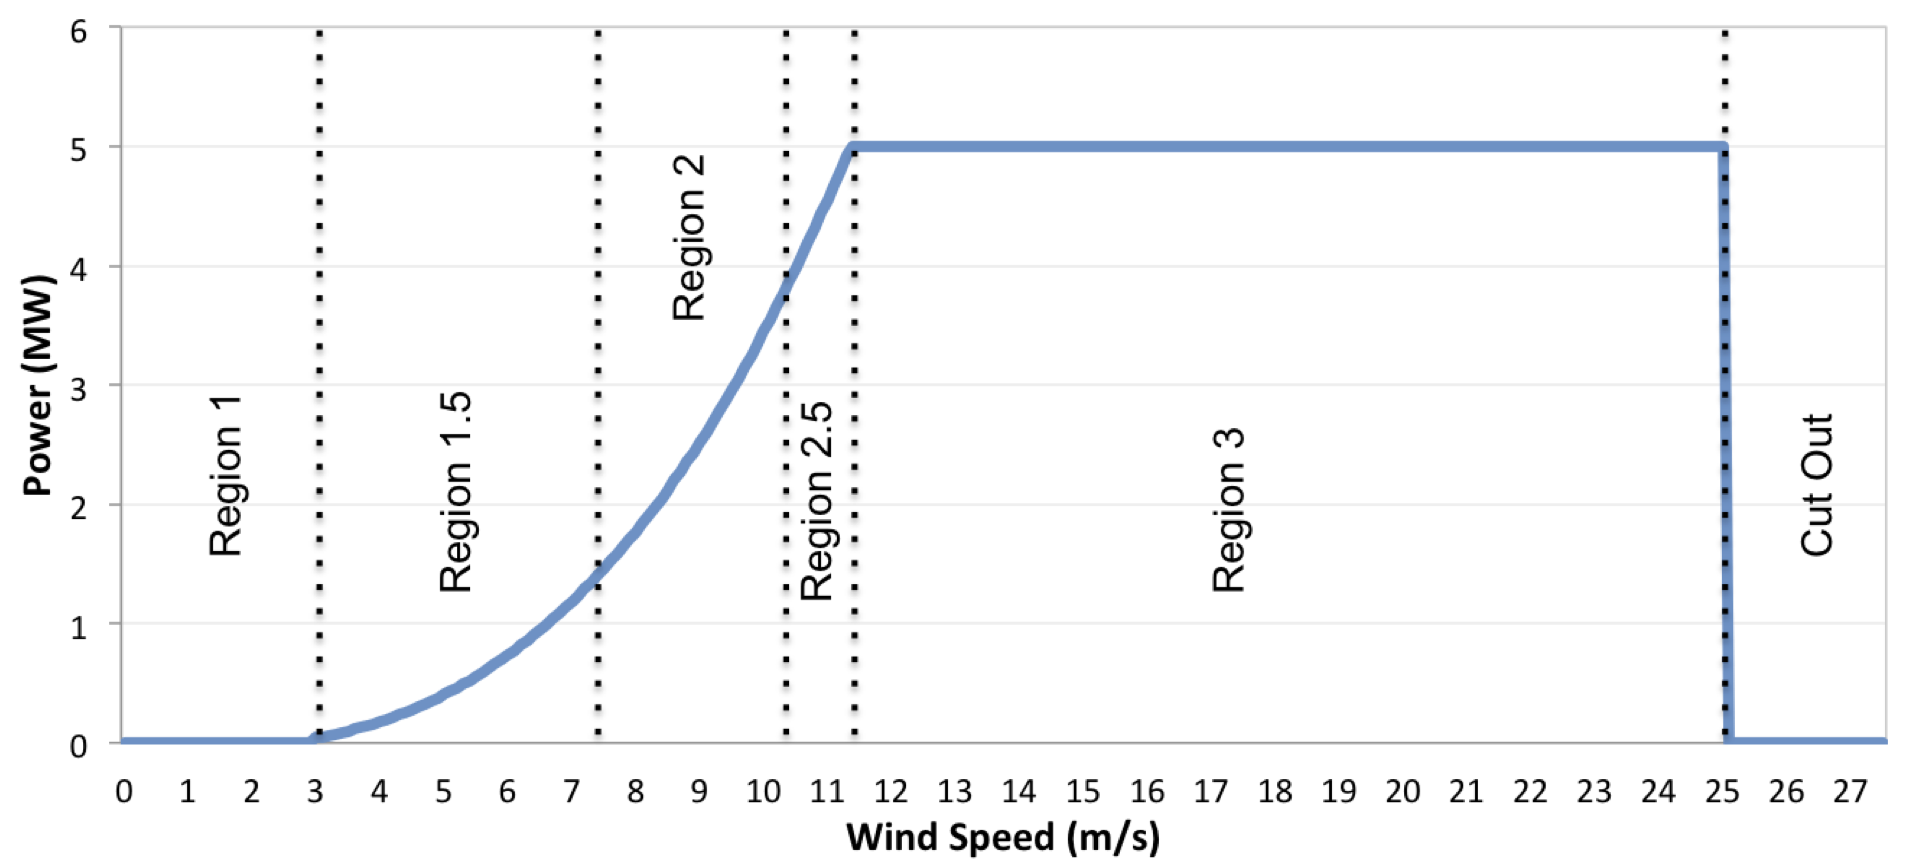
\includegraphics[width=\linewidth]{Figures/ch1Figures/fig1-6.png}
	\caption{Steady state behavior of the NREL 5-MW.\cite{jonkman2009}}
	\label{fig1-6}
\end{figure}

In region 2, deviations from the steady state power curve result in decreased aerodynamic efficiency and decreased power production.  By tracking the power curve more closely in this region the power production of the turbine can be increased.  In region 3, deviations from the steady state power curve cause higher loads on the mechanical components of the turbine and fluctuations in the power output of the turbine.  By tracking the power curve more closely the peak mechanical loads and fluctuation in power production can be reduced.

Reducing peak mechanical loads has several advantages.  It reduces wear and tear on the turbine$'$s mechanical components, thereby reducing the long-term repair and maintenance costs.  It can also lead to lower turbine-manufacturing costs or increased power production.  Reductions in manufacturing costs are achieved by designing and sizing the turbine components based on the reduced loads.  Alternately, increased power is achieved by ``growing the rotor''.  Which means to increase the size of the turbine blades until the loading on the turbine components matches the original design loads.

Reducing the power fluctuations in region 3 can also be used to increase power production without any physical changes to the turbine.  In part, the rated power of a turbine is set by the limitations of the turbine$'$s power electronics.  If improvements in wind turbine control can reduce deviations from rated power then the turbine can safely operate at a higher rated power without fear of overloading the power electronics.  This technique is currently being used by General Electric with its WindBOOST control system. The WindBOOST control system update allows the GE 1.5 MW wind turbine to operate at a rated power of 1.6 MW without any changes to the turbine hardware. \cite{GE2009}



%----------------------------------------------------------------------------------------
%	SECTION 5
%----------------------------------------------------------------------------------------

\section{Dissertation Outline}

Chapter \ref{Chapter2} investigates using a wind turbine as a sensor. It discusses the sensors that are present on a typical wind turbine and how sensor data can be used to gather useful information for feed forward control. Much of the chapter focuses on using turbine dynamics to estimate wind speed and convection velocity. Chapter \ref{Chapter2} also discusses the accuracy that can be expected from such estimates and discusses some of the factors that influence accuracy. 

In Chapter \ref{Chapter3}, a feed forward optimum pitch control scheme is introduced and investigated. In this control scheme an upwind is used as a wind speed sensor. Wind speed measurements are passed from the upwind turbine to a feed forward controller on a downwind turbine. The downwind turbine uses the knowledge of incoming wind speed to proactively adjust turbine blade pitch, potentially improving energy capture and reducing damage to the turbine. The control scheme is investigated through three rounds of simulation using the NREL FAST turbine simulation tool. The initial round of simulations uses a simplified idealistic model of the two turbine system, while the subsequent rounds systematically incorporate complicating factors that a real world system would encounter.  

Chapter \ref{Chapter4} investigates the benefits and feasibility of derating a downwind turbine based on a feed forward signal from an upwind turbine. Several derating strategies from literature are investigated to determine which is most feasible for feed forward control. The effects of derating on turbine loading and rotor overspeeds are examined. The transition into and out of derated mode is also investigated, as well as ways to mitigate undesirable turbine behavior during the transition. A feed forward selective derating scheme based on these findings is then developed. The performance of that feed forward control system is tested and evaluated using a series of FAST simulations. The FAST simulation results are promising, but it is determined that testing Feed Forward Derating Control with a different and more sophisticated wind turbine simulation tool would be beneficial.
  
Chapter \ref{Chapter5} is a verification and validation study of SOWFA (Simulator fOr Wind Farm Applications), a wind farm simulation tool. FAST must model a single turbine at time, but SOWFA can model a group of wind turbines as well at the atmospheric flow field surrounding those turbines. This gives SOWFA several advantages over FAST when modeling a two turbine system with feed forward control. However, SOWFA is much more computationally expensive than FAST and is less established in the wind turbine community. In Chapter \ref{Chapter5} the NREL 5-MW rotor is simulated using SOWFA, OVERFLOW2 and FAST. The results from these fundamentally different simulation tools are compared to see how well they agree. In addition, the chapter evaluates how near-rotor grid resolution and near-rotor grid length affect SOWFA simulation results. The results shown in Chapter \ref{Chapter5} increase confidence in SOWFA and provide guidance about how to properly tune and use SOWFA.

In Chapter \ref{Chapter6}, Feed Forward Derating Control is simulated and evaluated using SOWFA. The first portion of the chapter documents background work required to simulate the control system in SOWFA. Sections discuss implementing the feed forward controller, tuning SOWFA's actuator line model, choosing an appropriate computational domain, and gust modeling in SOWFA. The second portion of the chapter documents SOWFA simulation results for two test cases. One test case that matches the conditions assumed for Chapter \ref{Chapter4} FAST simulations, and one test case where turbine wake effects are prominent. In each test case a two turbine system is subjected to a large gust. The behavior of the upwind turbine, a downwind turbine without feed forward control, and a downwind turbine with Feed Forward Derating Control are compared and analyzed.

Chapter \ref{Chapter7} summarizes the dissertation and presents areas for future work.
